
\begin{definition}[Morse-datum]
	A \textit{Morse-Datum} is a quadrupel $\mathfrak{A}^{\alpha}=(M^{\alpha},f^{\alpha},g^{\alpha},\mathfrak{o}^{\alpha})$, where $M^{\alpha}$ is a closed orianted manifold, and $f^{\alpha}$ is a Morse function that is Morse Smale with respect to $g^{\alpha}$ and $\mathfrak{o}^{\alpha}$ is an oriantation of the unstable manifolds. 
\end{definition}
\begin{definition}[Transvers map]
	For two Morse-data $\mathfrak{A}^{\alpha},\mathfrak{A}^{\beta}$ we call a smooth map $h^{\beta\alpha}:M^{\alpha}\to M^{\beta}$ \textbf{transversal}, if for all $x\in \Crit(f^{\alpha})$ and $y\in\Crit(f^{\beta})$
	\begin{align}
		h^{\beta\alpha}|_{W(x\to)}\transcap W(\to y).
	\end{align} For the set of all such maps we write $\mathcal{F}(\mathfrak{A}^{\alpha},\mathfrak{A}^{\beta})$. 
	
	Finally we write $W_{h^{\beta\alpha}}(x,y):=W(x \to)\cap ({h^{\beta\alpha}})^{-1}(W(\to y))$.
\end{definition}
\begin{prop}
	Let $h^{\beta\alpha}\in \mathcal{F}(\mathfrak{A}^{\alpha},\mathfrak{A}^{\beta})$. Then for all $x\in \Crit(f^{\alpha})$ and $y\in\Crit(f^{\beta})$ the set $W_{h^{\beta\alpha}}(x,y)$ is a smooth oriented manifold of dimension $\ind(x)-\ind(y)$.
\end{prop}
\begin{proof} \todo{add details}
	By the transverse intersection, we have that $W_{h^{\beta\alpha}}(x,y)$ is an submanifold of $W(x \to)$ whith codimension of $W_{h^{\beta\alpha}}(x,y)$ in $W(x \to)$ equal to the codimension of $W(\to y)\subseteq M^{\beta}$. Compare \cite{Hirsch1994} Theorem 4.4 page 22. The differential of $h$ can be defined to be a map into the normal bundle $NW(\to y)$ . Hence we have the horizontally exact sequence:
	
	% https://tikzcd.yichuanshen.de/#N4Igdg9gJgpgziAXAbVABwnAlgFyxMJZABgBoBGAXVJADcBDAGwFcYkRiQBfU9TXfIRTkK1Ok1bsAKgHUA+sAAWAPWAAdNQCMYOeqQ1M0i+ly4AKAB6kAngEpuvEBmx4CRAEyiaDFm0QhZMwACCyCNHAgg+x4+F0EiAGYvcV92ADkZM3DIuwdYgTcUABZkn0l-ThinflchZCTiMTK-AIBZbjEYKABzeCJQADMAJwgAWyQyEAikcirhsZmaacR3OZHxlaWIJAS1hcQkqe3EIr2NzyOkAFZvCRaNKCwBgaCVdS0dPQNGIxM8kHmGxulwOt1S-g0aCwHS4QA
	\begin{tikzcd}
		&                                        &                                                              & TM \arrow[d, "\pi"] &   \\
		0 \arrow[r] & {TW_{h^{\beta\alpha}}(x,y)} \arrow[r] & TW( x \to ) \arrow[r] \arrow[ru, "{\diff h^{\beta\alpha}}"] & NW(\to y) \arrow[r] & 0
	\end{tikzcd}
	Now $TW(x \to)$ is oriented. Similar to the proof of lemma 7.30 in \cite{Seez2024} we can contract $W(\to y)$, by which we obtain a isomorphism between $NW(\to y)\cong T(y\to)$ and therby an orientation. Hence we can induce an orientation on $W_{h^{\beta\alpha}}(x,y)$ such that the exact sequence above is orientatino preserving (fiberwise). The codimension of $W_{h^{\beta\alpha}}(x,y)$ in $W(x \to)$ equals the codimension of $W(\to y)\subseteq M^{\beta}$ and thereby the dimension of $W_{h^{\beta\alpha}}(x,y)=\ind(x)-\ind(y)$.
\end{proof}
\begin{definition}
	We call $C(\mathfrak{A} {\alpha})$ the Morse chain group corresponding to the morse datum $\mathfrak{A}^{\alpha}$. Then by the proposition bevore we have that if $\ind(x)=\ind(y)$ we get a zero-dimensional oriented manifold $W_{h^{\beta\alpha}}(x,y)$. We define $n_{h^{\beta\alpha}}(x,y)$ to be the oriented count of the points. Then we define a map
	\begin{align}
		h_*^{\beta\alpha}: C(\mathfrak{A}^{\alpha}) & \to C(\mathfrak{A}^{\beta}) \\
		x & \mapsto \sum_{\{y|\ind(y)=\ind(x)\}}n_{h^{\beta\alpha}}(x,y) y
	\end{align}
\end{definition}
\begin{example}
	Let $h:S^2 \to S^2$ be the function, that deforms the sphere into the wiener sausage. Then on the Sphere and the sausage use the hight function and the standart induced metric (from $\mathbb{R}^3)$. Finally orient the tangend spaces of the unstable manifolds as shown in figure \ref{fig: induced functions sphere to wiener}. In the bottom of that figure one can inspect the pulled back (un-)stable manifolds via $h$. This leads to the map of chain complexes, where the left side is the chain complex corresponding to the Sphere and the right side to the sausage. The induced maps are given horizontally: 
	\begin{center}
		% https://tikzcd.yichuanshen.de/#N4Igdg9gJgpgziAXAbVABwnAlgFyxMJZABgBpiBdUkANwEMAbAVxiRGJAF9T1Nd9CKMgEYqtRizYAdKQzpgA5gxgACNCpkAneUtbde2PASJkATGPrNWiEDLmLlK4hqnaHeniAyGBJ0gGYLCWtbWR1HOBc3XS5Pb35jIVIAFiCrNg59Lz4jQWRTcjTJG0y4nN8UAtFqS2LQ+101AHJSAEcmqPCPAwS8gvMa4Okw9xVNDq0u2J7cogLAwfSbOy6VOAnXKaz42cqUopDMsRgoBXgiUAAzTQgAWyQyEBwIJGEs67vX6mekU3eb+6IApPF6Ifz-T5g76g5IQwEAVmhSAAbHCkAAOJGIACcaMQwixyMWdTQMludDQcGeKmEMgAxlAIDhmgBqGkuBlMlTtaYgD6A4E-RAAdmJh15-KQ-ixmPESxAcDJFKpEDWTQlAJRWNFCoAFlhLjgkABaaVPOhYBhscmUn5i4bknCaLAAD2AaCaSttquN4xcMnaLhtKpULPGnA1kKJIKQwrxOqF6PjMuocH1hpNZpwFqtNmDdrldT9XpDR04QA
		\begin{tikzcd}
			0 \arrow[d]                                                              &  & 0 \arrow[d]                                                                                                   \\
			\langle p \rangle \arrow[d] \arrow[rr, "p\mapsto 1\cdot p'+ 1 \cdot q'"] &  & {\langle p',q' \rangle} \arrow[d, "\begin{smallmatrix}p'\mapsto -r' \\q' \mapsto +r'\end{smallmatrix}", maps to, shift left=3] \arrow[d] \\
			\langle 0 \rangle \arrow[d] \arrow[rr, "0"]                              &  & \langle r' \rangle \arrow[d] \arrow[d, "r' \mapsto 0", maps to, shift left=3]                                 \\
			\langle s \rangle \arrow[d] \arrow[rr, "s\mapsto s'"]                    &  & \langle s' \rangle \arrow[d]                                                                                  \\
			0                                                                        &  & 0                                                                                                            
		\end{tikzcd}
	\end{center}
\end{example}
\begin{figure}
	\centering
	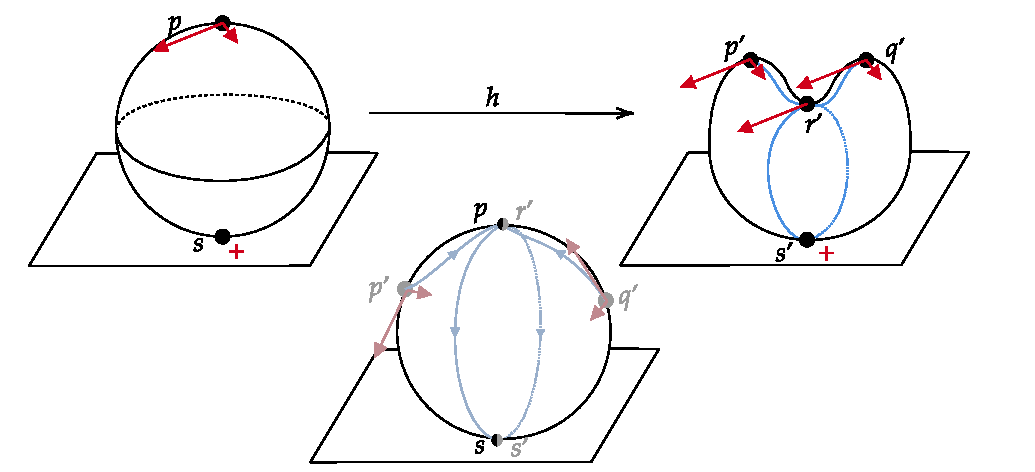
\includegraphics[width=0.8\linewidth]{Text/Pictures/Functoriality/induced function.pdf}
	\caption{The induced (un-)stable structures}
	\label{fig: induced functions sphere to wiener}
\end{figure}
\begin{remark}
	By definition we have that the map $\id _*^{\alpha \alpha}=id_{C(\mathfrak{A}^{\alpha})}$.
\end{remark}
\begin{remark}
	The plan now is to proof that :
	\begin{enumerate}
		\item $h_*^{\beta\alpha}$ is a chain map.
		\item $h_*$ is homotopic invariant in the following sense: Suppose we have the Morse data $\mathfrak{A}^{\alpha},\mathfrak{A}^{\beta},\mathfrak{A}^{\gamma},\mathfrak{A}^{\delta}$, where $M^{\alpha}=M^{\gamma}$ and $M^{\beta}=M^{\delta}$. Assume now that $h^{\delta\gamma}\in \mathcal{L}(\mathfrak{A}^{\alpha},\mathfrak{A}^{\beta})$ is homotopic to $h^{\beta\alpha}\in\mathcal{L}(\mathfrak{A}^{\gamma},\mathfrak{A}^{\delta})$. Then  $h_*^{\delta\gamma}\Phi_*^{\gamma\alpha}$ is homotopic to $\Phi_*^{\delta\beta}h_*^{\beta\alpha}$.  \todo{wad is den datt Phi hier??}
	\end{enumerate}
\end{remark}
\begin{figure}
	\centering
	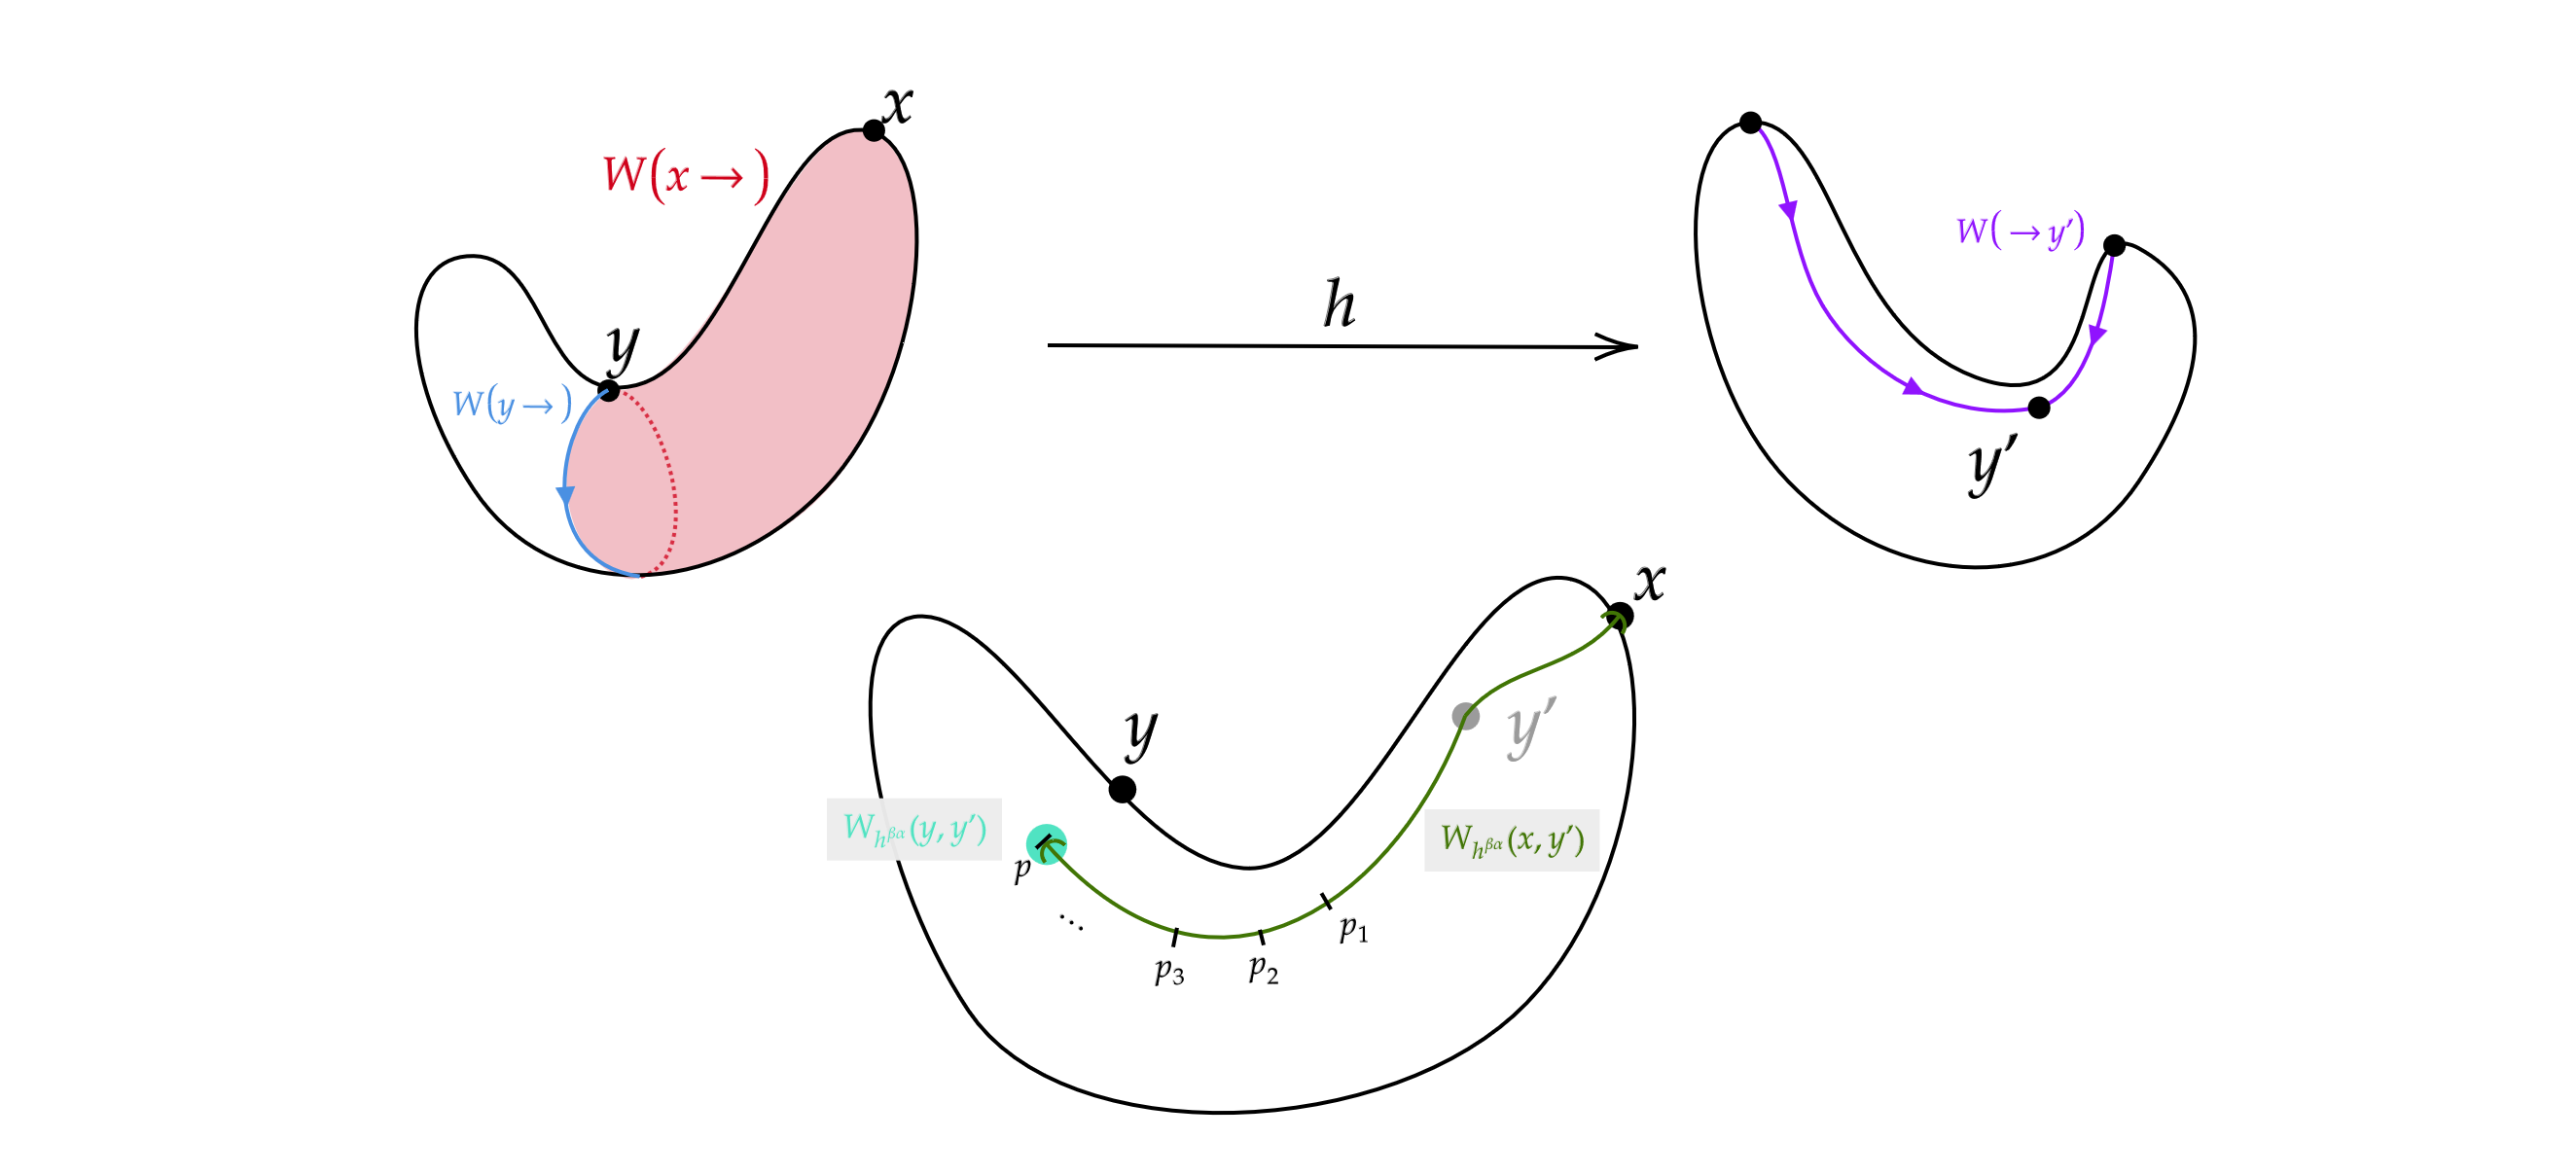
\includegraphics[width=1\linewidth]{Text/Pictures/Functoriality/Compactness .png}
	\caption{Compactness of $\Whab(x,y')$}
	\label{Compactness of Whab}
	In this figure $h$ is a mostly vertical deformation and a little bit of a rotation. In the lower picture one can see the pulled back structure and the space $\Whab$. The sequence $p_k$ shows the second case, i.e. the braking of the orbits in the domain.
\end{figure}
\begin{prop}
	Let $h^{\beta\alpha}\in \Lab$ ,$x\in \Crit(f^{\alpha}),y'\in \Crit(f^{\beta})$ with $\ind(x)-1=\ind(y')$. Let $p_k$ be a sequence in $\Whab(x,y')$ be a sequence that approaches $p\in M^{\alpha}$. Then either one of the following is true:
	\begin{enumerate}
		\item $p\in \Whab(x,y')$.
		\item There exists $y\in \Crit(f^{\alpha})$, with $\ind(y)=\ind(y')$ such that $p\in \Whab(y,y')$. The orbits through $p_k$ break to orbits \todo{break to orbits genauer definieren} $(u_1,...,u_l)$ as $k\to \infty$ with $u_1\in W(x\to y)\slash \R$.
		\item There exists $x'\in\Crit(f^{\beta})$, with $\ind(x)=\ind(x')$ such that $p\in \Whab(x,x')$. Furthermore, the orbits through $h^{\beta\alpha}(p)$ break to the orbits $(u'_1,...,u'_l)$ as $k\to \infty$ where $u'_l\in W(x'\to y')\slash \R$.
	\end{enumerate}
\end{prop}
\begin{proof}
	Since the sets $\Whab(x,y'),~\Whab(y,y')$ and $\Whab(x,x')$ are disjoint, the cases are disjoint aswell. There are only finitly many critical points and hence we can restrict to a subsequence such that all $p_k\in W(x\to b)$ for some fixed $b\in \Crit(f^{\alpha})$. By the broken orbits lemma \ref{lem. Broken orbits lemma} we know that there exist $y,a\in \Crit(f^{\alpha})$ such that $x\succeq y\succeq a\succeq b$ and $p\in W(y\to a)$. Since $x\succeq y$ we have that $\ind(x)=\ind(y)$ only in the case of $x=y$. That is shown in \ref{cor: lambda lemma flow lines have decreasing index}. In the same way we again restrict the sequence, such that $h^{\beta\alpha}(p_k)$ lives in $W(a',y')$ for some fixed $a'\in \Crit(f^{\beta})$. Then $h^{\beta\alpha}\in W(b',x')$ with $a'\succeq b'\succeq x'\succeq y'$ and $\ind(x')=\ind(y')$ only if $x'=y'$.
	
	Now assume that $p\nin W(x\to)$ and $h^{\beta\alpha}(p)\notin W(\to y')$. Then $p\in W(y\to)$ and $h^{\beta \alpha}(p)\in W(\to x')$, i.e. $p\in \Whab(y,x')$. But since $x\neq y$ and $y'\neq x'$ they need to be of lower, respectively higher index and hence the index difference is lesser then minus one. This yields a contradicting since then $\Whab(y,x')=\emptyset$. So only three possibilities are left, where the first one is the first case. So assume $p\nin \Whab(x,y')$. 
	
	If $p\in \Whab(x,x')$ then by assumption we have that $\ind(x')\geq \ind(y')$. Hence $\dim(\Whab(x,x'))\leq 0$ and since $p$ exists it needs to be zero telling us that $\ind(x)=\ind(x')$. The statement about the breaking orbits is a reformulation of \ref{lem. Broken orbits lemma}. This shows the second part. 
	A similar calculation shows the third part.
\end{proof}

\begin{lemma}($\lambda-$lemma )
	Let $W\subseteq M$ be an immersed submanifold of $M$ and let $p$ be a hyperbolic fixpoint of a diffeomorphism $\phi$ on $M$ with $\dim W(p \to)=r$ for ${0<r<m=\dim M}$. Let $N$ be an injective immersed submanifold of $M$ that is invariant under $\phi$ and has a point of transverse intersection $q$ with $W(\to p)$. Then for any $r-$cell neighbourhood $D$ of $q$ in $N$ and any $r-cell$ neighbourhood $B$ of $p$ in $W(p\to))$ there is a smaller cell $\tilde{D}\subset D$ and an $n\in \N$ such that $B$ is $\epsilon~C^1$-close to $\phi^m(D)$ for all $m>n$
\end{lemma}
\begin{proof}
	In \ref{thm: lambda Lemma} we proofed the same with the only difference, that we defined the $r-$cell $D$ arbitrary. We now want to show that this $r-$cell can be defined to be the image of a moved smaller cell of a given $r-cell$. So lets inspect the already given proof:
	
	We started by moving the point of transverse intersection $q$ closer to the fixpoint by applying the diffeomorphism to it. Then we defined an neighbourhood $D_0$ of that moved point in the stable manifold (compare \ref{eq: proof lambda lemma small neighbourhood}). Here we were able to get a hold of the inclination. Then we moved $D_0$ via applying the isomorphism closer to the fixed point and restricted it to the dimension of the unstable manifold. This restriction we can refine as follows: First we define $D_{n^2}$ to be the moved $D_0$. Lets say we moved $q$ $n-$times. In other words $q\in \phi^{-n}(D_{n^2})$ Then there exist a small $r-$cell neighbourhood of $q$ that lives in $D \cap \phi^{-n}(D_{n^2})$. That is because $ \phi^{-n}(D_{n^2})$ is an in $N$ open neighbourhood of $y$, hence $\phi^{-n}(D_{n^2}) \cap D$ is open in $D$. Hence we can find a ball around $y$ in $D$ that is contained in the intersection. We call that $r-$cell $\tilde{D}$. Then $\phi^n(\tilde{D})$ is an $r-$dimensional subset of $D_{n^2}$ and the rest of the proof can be done with that subset. All arguments work, as that subset is transverse to $W(\to p)$. 
\end{proof}
\begin{lemma}[Gluing on ends] \label{lem: gluing on ends}
	Let $f:M\to \R$ be a Morse function, $\mathfrak{g}$ a metric, and $y \in \Crit(f)$. Let $m=\dim(M)$ and suppose $D^{\ind(y)}$ and $E^{m-\ind(y)}$ are embedded discs of dimension $\ind(y)$ and $m-\ind(y)$ such that $D^{\ind(y)}\transcap W(\to y)$ and $E^{m-\ind(y)} \transcap W(y \to)$. Assume furthermore that the intersections consist of only one point $\{u\}=D^{\ind(y)}\cap W(\to y), \{v\}=E^{m-\ind(y)} \cap W(y \to)$.Then there exists an $R_0>0$ and an injective map $\rho:[R_o,\infty)\to M$ such that $g(\frac{\diff}{\diff R}\rho (R),-\grad_g(f))\neq 0$, and $\phi_{-R}(\rho(R))\in D^{\ind(y)}$, and $\phi_R(\rho(R))\in E^{m-\ind(y)}$. We have the limits:
	\begin{equation*}
		\lim_{R\to\ \infty}(\rho(R))=y, \quad \quad\lim_{R\to\ \infty}\phi_{-R}(\rho(R))=u,\quad \quad \lim_{R\to\ \infty}\phi_{R}(\rho(R))=v. 
	\end{equation*}
	Finally, there exists smaller discs $D'\subseteq D^{\ind(y)}$ and $E'\subseteq E^{m-\ind(y)}$ such that no orbit through $D'\setminus \cap_{R\in[R_0,\rho(R)}\phi_{-R}(\rho(R))$ intersects $E'$.
\end{lemma}
\begin{proof}
	First we define $B^u\subseteq W(y \to)$ and $B^s\subseteq W(\to y)$ to be closed balls containing $y$. Denote 
	\begin{equation*}
		\phi_R(D^{\ind(y)}:=D^{\ind(y)}_R, \text{ and }\phi_{-R}(E^{m.\ind(y)}):=E^{m-\ind(y)}_{-R}.
	\end{equation*} 
	By the $\lambda-$lemma we can conclude, that there exists a smaller cell $D'\subseteq D^{\ind(y)}_R$ such that $D'$ is $\epsilon~C^1-$close to $B^u$. Similar by using the lemma for $-f$ we can find a $E'\subseteq E^{m-\ind(y)}_{-R}$ that is $\epsilon'~\C^1-$close to $B^s$.  Therefore, by definition we get the following maps:
	\begin{align*}
		\phi^R:B^u&\to D'_R; \quad \phi^{R}(q)=(\phi^R_s(q),\phi^R_u(q)) \\
		\psi^R:B^s& \to E'_R;\quad \psi^R(p)=(\psi^R_s(p),\psi^r_u(p))
	\end{align*}
	Here we used a coordinate notation for the maps, where that chart locally splits into the (un-)stable manifolds. This can be done by the local (un-)stable manifold theorem. In other words the maps are given as follows:
	\begin{align*}
		\phi^R_s:B^u \to W(\to y),\quad &   \quad    \phi^R_u:B^u\to W(y\to )\\
		\psi^R_s:B^s\to W(\to y), \quad & \quad \psi^R_u:B^s\to W(y\to ).
	\end{align*}
	By the closeness conditions those maps satisfy: 
	\begin{align*}
		&\left\lVert
		\begin{pmatrix}
			0\\
			q
		\end{pmatrix}
		-
		\begin{pmatrix}
			\phi^R_s(q)\\
			\phi^R_u(q)
		\end{pmatrix}
		\right\rVert < \epsilon , \quad &
		\left\lVert
		\begin{pmatrix}
			0\\
			1
		\end{pmatrix}
		-
		\begin{pmatrix}
			\diff \phi^R_s(q)\\
			\diff \phi^R_u(q)
		\end{pmatrix}
		\right\rVert < \epsilon \quad \forall q\in B^u\\
		& \left\lVert
		\begin{pmatrix}
			p\\
			0
		\end{pmatrix}
		-
		\begin{pmatrix}
			\psi^R_s(p)\\
			\psi^R_u(p)
		\end{pmatrix}
		\right\rVert < \epsilon, \quad &
		\left\lVert
		\begin{pmatrix}
			1\\
			0
		\end{pmatrix}
		-
		\begin{pmatrix}
			\diff \psi^R_s(p)\\
			\diff \psi^R_u(p)
		\end{pmatrix}
		\right\rVert < \epsilon \quad \forall q\in B^s
	\end{align*}
	Now after choosing $\epsilon$ small enough we can make sure that $\im \phi^R_s$ lives in $B^s$ and $\im \psi^r_u\subset B^u$. Furthermore, for $\epsilon$ small enough we can invert $\phi^R_s$ and $\psi^R_u$. Then we can define the compositions locally:
	\begin{align*}
		G_R:B^u\supseteq \im \phi^R_s \to B^s ; q \mapsto \phi^R_s \circ (\phi^R_u)^{-1}(q)\\
		F_R: B^s \supseteq \im \psi^r_u \to B^u; p \mapsto \psi^R_u \circ (\psi^R_s)^{-1}(p)
	\end{align*}
	Now $D'_R$ and $E'_R$ are the graph of $G_R$ respectively of $F_R$. To see this just notice:
	\begin{equation*}
		(q,G_R(q))=(q,\phi^R_s ( \underbrace{(\phi^R_u)^{-1}(q)}_{:=\tilde{q}}))=(\phi^R_u(\tilde{q}),\phi^R_s(\tilde{q})=\phi^R(\tilde{q})
	\end{equation*}
	
	And analogously for $F_R$. Now we want to intersect the graphs and even more: we want to show that they intersect only in one point. First we notice, that the intersection of the graphs, is a fixpoint of $F_R\circ G_R$. We know already that the graphs intersect, since $B^s$ and $B^u$ intersect transversal and by the stability theorem \ref{thm: stability theorem} $E'_R$ and $D'_R$ this propertie carries over to the graphs. For the uniqueness we realize that $F_R\circ G_R$ is a contraction and by the Banach fixpoint theorem we get uniquness:
	\begin{align*}
		\norm{\diff (F_R\circ G_R)|_q}&=\norm{\diff (\psi^R_u \circ (\psi^R_s)^{-1}\circ \phi^R_s \circ (\phi^R_u)^{-1})|_q} \\
		&=\norm{\diff \psi^R_u|_{(\psi^R_s)^{-1}\circ G_R(q)}\circ \diff ((\psi^R_s)^{-1})_{G_R(q)}\circ \diff (\phi^R_s)_{(\phi^R_u)^{-1}(q)}\circ \diff (\phi^R_u)^{-1}|_q}\\
		&\leq \epsilon^2\norm{\diff ((\psi^R_s)^{-1})_{G_R(q)}}\cdot \norm{\diff (\phi^R_u)^{-1}|_q} \\
	\end{align*} Now we can use the inverse function theorem and the triangle inequality: First define the matrix $S:=\diff ((\psi^R_s)^{-1})_{G_R(q)}$.
	\begin{align*}
		1=\norm{(S-S\cdot (1-S^{-1}))}\geq \norm{S}-\norm{S}\cdot \underbrace{\norm{1-S^{-1}}}_{<\epsilon} 
	\end{align*} Hence $\norm{S}\leq 1-\epsilon$ Similar we get a hold of $\norm{\diff (\phi^R_u)^{-1}|_q}$ to conclude:
	\begin{align*}
		\norm{\diff (F_R\circ G_R)|_q}\leq \frac{\epsilon^2}{(1-\epsilon)^2}.
	\end{align*}Hence the derivative is strictly less then a number less then one if $\epsilon$ is less then a half. this gives a contraction and thereby a unique fix point. Now collect what we have done: 
	
	For this whole construction we need the epsilon small enough. The $\lambda-$lemma tells us, that there is an $R_0$ such that for all $R>R_0$ this construction works. So if we fix the $\epsilon$ and thereby $R_0$ once, we get such an intersection point for each $R>R_0$. With this we define the map $\rho(R)$ that satisfies all required properties:
	
	First the map is differentiable: That is because the maps $\Phi_R$ and $\Psi_R$ smoothly depend on $R$. This can be seen as they are a composition of the maps that come out of the $\lambda-$lemma, and in that lemma they are the composiontin of smooth maps. (Applying the diffeomorphism and a projection). Hence the maps $F_R$ and $G_R$ smoothly depend on $R$ and thereby the contraction $F_r\circ G_R$. Now we inspect the function $(R,x)\mapsto x-F_R\circ G_R$. The level zero set of this map gives our intersection points with respect to $R$ and since
	\begin{align*}
		\frac{\partial (x-F_R\circ G_R)s}{\partial x}\neq 0 \, ,
	\end{align*} we conclude by the implicit function theorem, that the map $\rho$ is smooth. 
	Assume that it would not be injective. For that we would need without restriction points in $D'$ and in $\phi_t(D')$ for $t>0$. But by the transversality and since $\dim(D')=m-\ind(y)$ this cannot happen.
	
	We need to show, that $\frac{\diff \rho}{\diff R}$ and $-\grad(f)$ are linearly independent. This however is clear since otherwise both discs need to be moved in the direction $-\grad(f)$ (or both in the  $+\grad(f)$ direction) which is not the case.   
	
	
\end{proof}
\begin{lemma}
If $N_p$ is defined as in the proof of theorem \ref{thm commuting connecting homomorphism}. Then $N_p$ is a tubular neighbourhood of $W(\to p)\cap M^c$
\end{lemma}
\begin{proof}
	First we inspect the boundary conditions of $N_p$ and make use of the lemma above. $f^{-1}(c)$ is a submanifold in $M$ that intersects $W(\to p)$ transversal since the gradient is orthogonal to level sets. This means, that 
	\begin{align*}
		T_xM=T_xf^{-1}(c)+T_xW(\to p)\quad \forall x\in W(\to p)\cap f^{-1}(c)
	\end{align*} and hence we have the inclusions
	\begin{align*}
		TN_xW(\to p)\hookrightarrow T_xf^{-1}(c)\hookrightarrow f^{-1}(c)\, .
	\end{align*} The last inclusion is induced from a chart. By doing this for all $x\in W(p\to)\cap f^{-1}(c)$ we have the normal over the intersection indluded into $f^{-1}(c)$. For each $x$ the normal bundle is of dimension $\lambda_p$ and hence for each $x$ we have a $\lambda_p$-dimensional disc $D^{\lambda_p}$. 
	Now let $y\in W(\to p)\cap M^c$. Then since $f(\phi_{-T}(y))$ increases for increasing $T$ and gets bigger then $c$, we know that $y=\phi_R(x)$ for sime $x\in W(\to p)\cap f^{-1}(c)$. Now we can map the embedded normal space of $x$ to $y$ via $\phi_R$. Or with the naming above: $\phi_R(D^{\lambda_p})$. \todo{das passt nicht: I now want to rescale this embedded disc. So for $v\in \partial B_{\epsilon'}(y)\subseteq\phi_R(D^{lambda_p})$ we can assume that $f(\phi_T(v))\leq a-\epsilon$. And by making $T$ big enough we can assume, that there is a smallest scaler $\lambda_v$ such that $f(\phi_T(\lambda_v\cdot v))=a-\epsilon$. By continuoty of the flow and $f$ we can assume, that $\lambda_v$ smoothly depends on $v$??? Mist nein dohc nicht}
	Now intersect $(f\circ\phi_T)^{-1}(a-\epsilon)\cap\phi_R(D^{\lambda_p})$ and pull it back to the normal. by first pulling it back via $\phi_R$. 
			 
	
	Furthermore, we inspect $f^{-1}(a-\epsilon)$ which is again a codimension one manifold that transversally intersects $W(p\to)$ and again in the intersection we can map the normal bundle of $W(p\to)$ into $f^{-1}(a-\epsilon)$. So now assume that the subset 
	\begin{align*}
	\{	x\in \phi_R(D^{\lambda_p})| f\circ \phi_T(x)\leq a-\epsilon\}
	\end{align*} is \textbf{not} starshaped. since its boundary is given by the smooth manifold $(f\circ\phi_T)^{-1}(a-\epsilon)\cap\phi_R(D^{\lambda_p})$ this means that 
\end{proof}
\begin{figure}
	\centering
	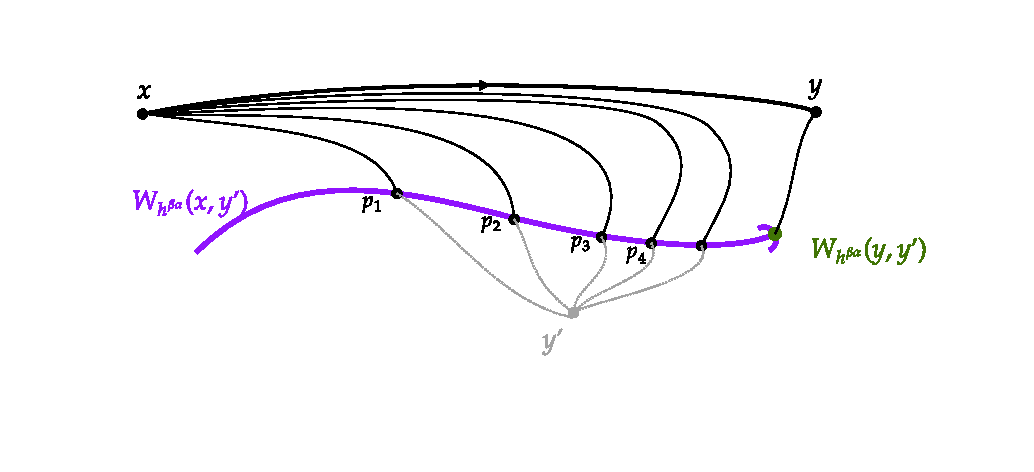
\includegraphics[width=0.7\linewidth]{Text/Pictures/Functoriality/Gluing on the boundary.pdf}
	\caption{The space $\Whab(x,y')$}
	\label{fig:whab(x,y')}
\end{figure}
\begin{prop}
	Assume that $h^{\beta,\alpha}\in \Lab$. Then for critical points $x,y\in \Crit(f^{\alpha})$ and $x',y'\in \Crit(f^{\beta})$, with $\ind(x)=\ind(x')=\ind(y)-1=\ind(y')-1$, there exists $R_0>0$ and gluing embeddings
	\begin{align*}
		\#^1&:(W(x,y)\slash \R) \times [R_0,\infty)\times (\Whab(y,y')\to \Whab(x,y')\\
		\#^2&: \Whab(x,x')\times [R_0,\infty)\times (W(x'\to y')\slash \R)\to \Whab(x,y') \,.
	\end{align*}
	Moreover, if $p_k\in \Whab(x,y')$ converges to $p\in \Whab(y,y')$, and the orbits through $p_k$ break as $(u_1,...,u_l)$ with $u_l\in (W(x\to y)\slash \R)$ then $p_k$ is in the image of $\#^1$. Analogously if $p_k$ converges to $p\in \Whab(x,x')$ and the orbits break to $(u_1,...,u_1')$ with $u_l'\in (W(x'\to y)\slash \R)$, then $p_k$ is in the image of $\#^2$ for $k$ big enough.
\end{prop}
\begin{proof} We denote the dimensions of $M^{\alpha}$ and $M^{\beta}$ with $m^{\alpha}$ and $m^{\beta}$
	First let $u\in W(x\to y)$ and $v\in \Whab(y,y')$. Now we can choose a disc $D^{\ind(y)}$ in $W(x\to)$ through $y$ and transverse to $W(\to y)$. In the same way we can find a disc $E^{m^{\alpha}-\ind(y)}$ through $v$ that is transverse to $W(y\to)$. Then from lemma \ref{lem: gluing on ends} we get the map $\rho$ and with that we define $\#^1(\gamma_u,R,v):=\phi_R(\rho(R))$ now this mapping \todo{}
\end{proof}